\documentclass{article}
\usepackage[utf8]{inputenc}
\usepackage{hyperref}
\usepackage{geometry}
%Mettere le foto sulla stessa
\usepackage{subcaption}
%lib img
\usepackage{natbib}
\usepackage{graphicx}
\hypersetup{
    colorlinks=true,
    linkcolor=red,
    filecolor=red,      
    urlcolor=red,
}
%impaginazione margini ecc...
\geometry{a4paper, top=3cm, bottom=3cm, left=2.5 cm, right=3.5cm }
\title{Script}
\author{a.daguanno1 }
\date{April 2021}

\begin{document}

\maketitle

\section{Introduction}
\section{Compiler}
\begin{itemize}
    \item\url{https://www.python.org/downloads/release/python-394/}
\end{itemize}
\section{Library Script - \textbf{Prgetto2}}
\subsection{Anaconda}
Anaconda è una distribuzione dei linguaggi di programmazione Python per il calcolo scientifico. Che mira a semplificare la gestione e la distribuzione dei pacchetti.
\\Racchiude in se il compilatore python, un pakage enviroment "Conda" che ci consente di istallare i package 
\begin{itemize}
    \item\url{https://www.anaconda.com/products/individual/download-success}
    \item\url{https://www.youtube.com/watch?v=UmORrAvr4pQ}
\end{itemize}
\begin{enumerate}
    \item Avviamo l'istallazione
    \item Avviamo poi Anaconda Navigator l'app istallata
    \item Cerchiamo una libreria andado sulla sinistra nella voce "Environments" e cercando ad es "numpy"
\end{enumerate}

\textbf{Creare il proprio environment}
\begin{enumerate}
    \item In Environmets in Anacoda Navigator cliccare si create in basso a sinistra 
    \item Inserire un titolo
    \item Cercare poi i package che si devono utilizzare nell'ambiente del progetto ed installarli 
    \begin{figure}[h!]
        \centering
        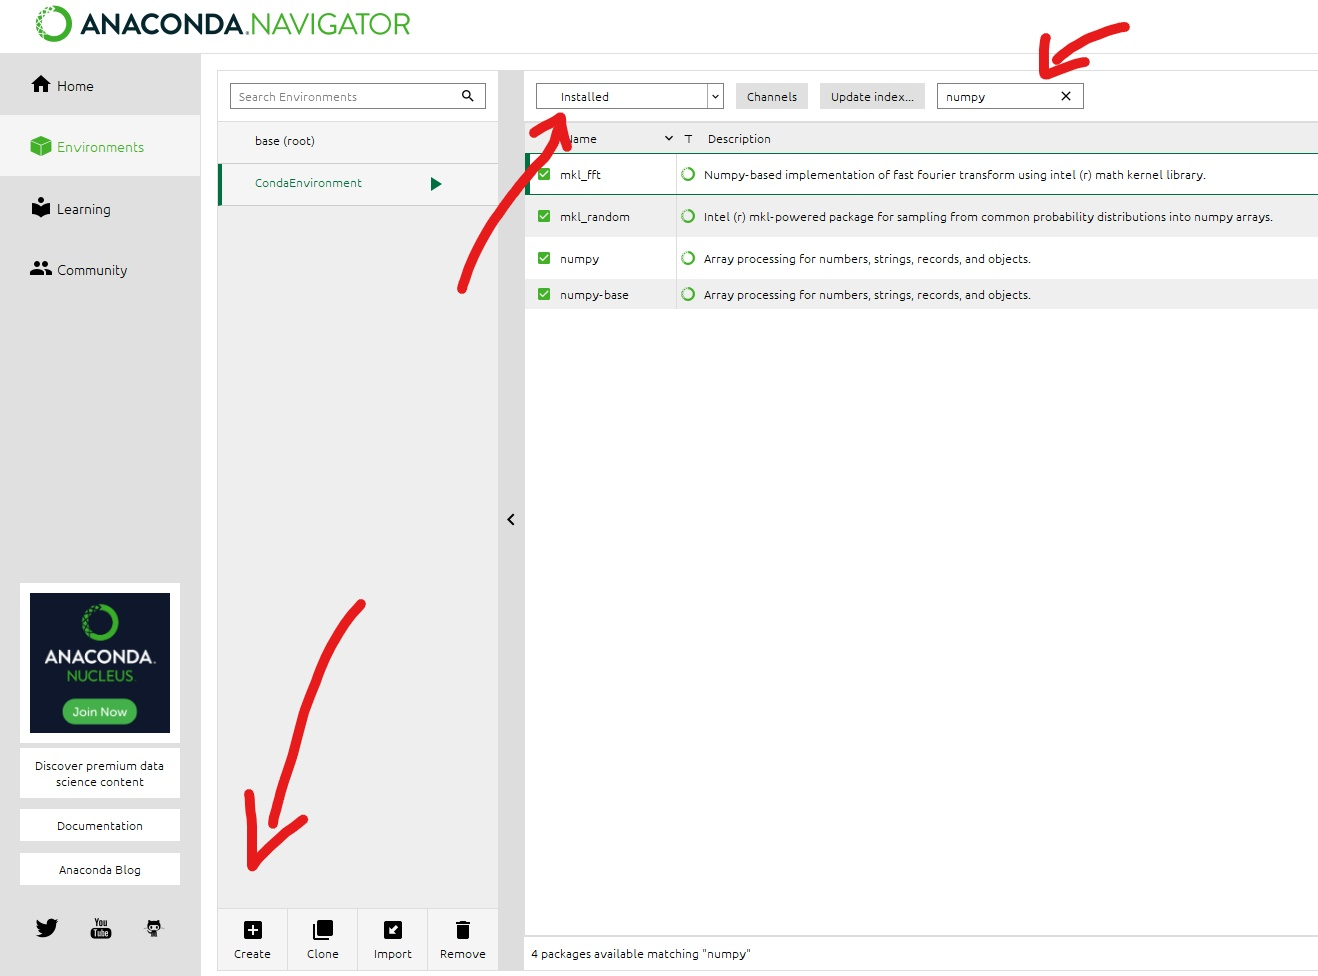
\includegraphics[scale= 0.1]{image/AncaondaEnvironmet.jpg}
        \caption{Anaconda Environments}
        \label{fig:my_label}
    \end{figure}
    \item dall'Ide poi configurare come interprete Conda ed il nome dell'environment che si è creato
     \begin{figure}[h!]
        \centering
        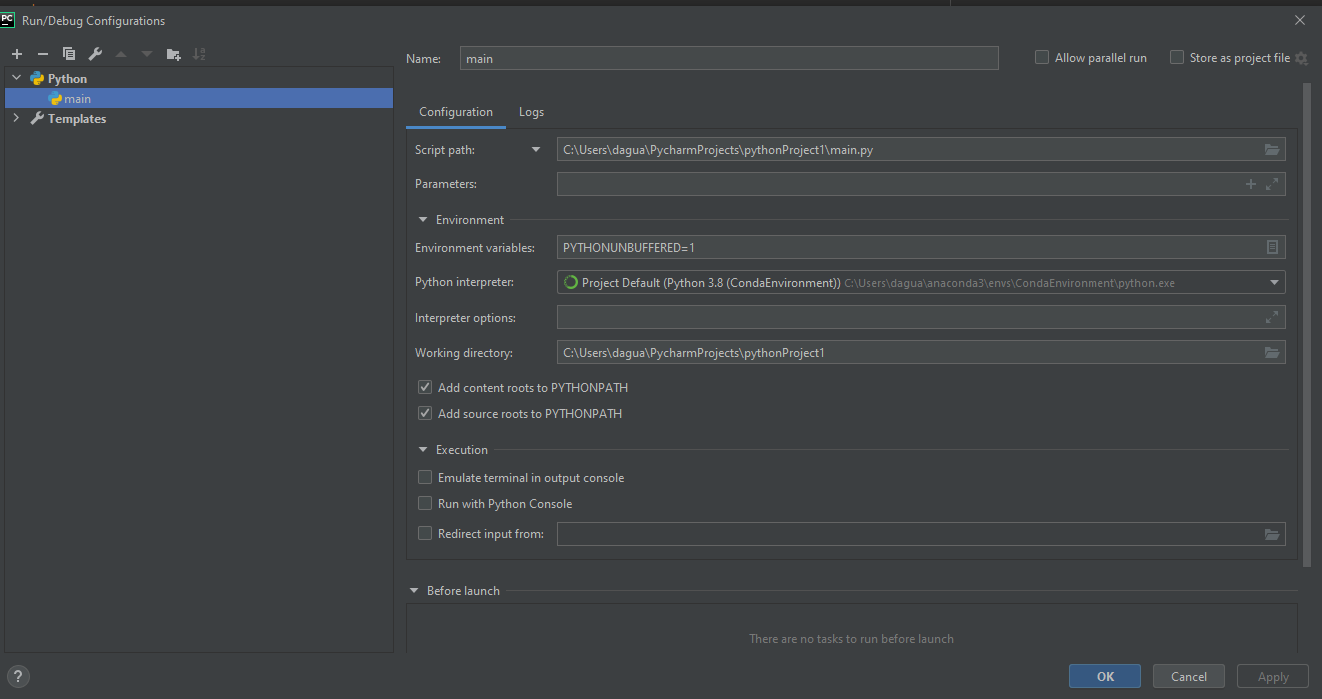
\includegraphics[scale= 0.2]{image/ideEnviroment}
        \caption{IDE Environments}
        \label{fig:my_label}
    \end{figure}
    \item Per \textbf{run} si va su edit configuration icon\textbf{ +} poi \textbf{python} selezionare Conda da \textbf{Python interpreter} dargli un nome e fare attenzione che "Environment variables" sia settata altrimenti creare un nuovo progetto facendo attenzione in fase di creazione di impostare correttamente l'interprete \textbf{Conda}
    \\In "Script Path" trovare inserire la path dello script che bisogna interpretare
     \begin{figure}[h!]
        \centering
        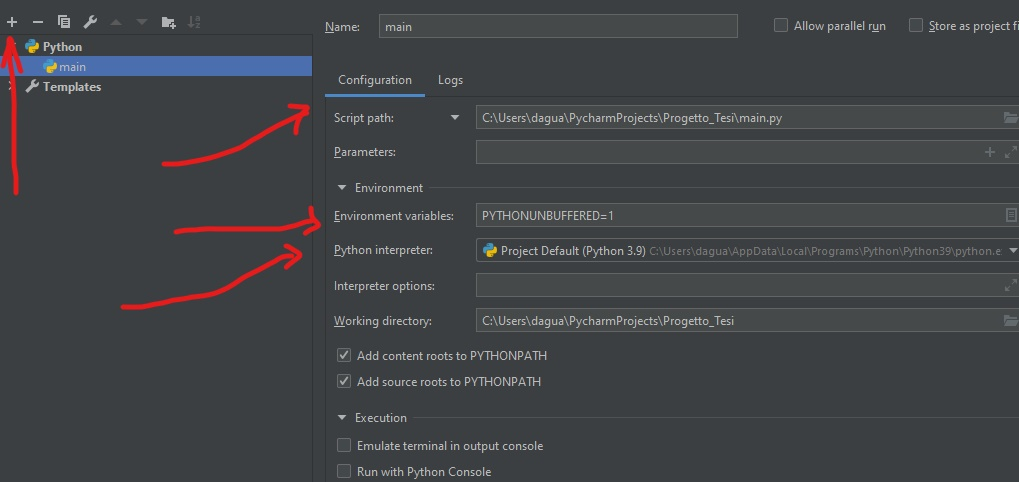
\includegraphics[scale= 0.2]{image/Screenshot (29)_LI.jpg}
        \caption{Porject Environments}
        \label{fig:my_label}
    \end{figure}
\end{enumerate}
\subsection{CSV Library}
INFO: \url{https://docs.python.org/3/library/csv.html}
\\La libreira \textbf{CSV} implementa classi per leggere e scrivere dati tabulari in formato CSV. Consente ai programmatori di dire "scrivere questi dati nel formato preferito da Excel" o "leggere i dati da questo file che è stato generato da Excel", senza conoscere i dettagli precisi del formato CSV utilizzato da Excel. I programmatori possono anche descrivere i formati CSV compresi da altre applicazioni o definire i propri formati CSV speciali.
\subsection{Librosa}
Per installare la libreria in Anaconda \url{https://anaconda.org/conda-forge/librosa}
\\Info: \url{https://librosa.org/doc/latest/index.html}
\\Libreria per leggere e manipolare un file audio

\subsection{Matplotlib}
Importiamo matplotlib per visualizzare l'ampiezza di un suono
\begin{figure}[h!]
        \centering
        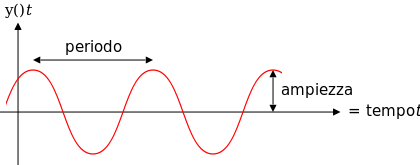
\includegraphics[scale= 0.2]{image/420px-Oscillazione_periodica.svg.png}
        \caption{Ampliezza di un suono}
        \label{fig:my_label}
    \end{figure}

\subsection{Numpy}
Importiamo numpy per la computazione numerica 
\subsection{Os}
INFO: \url{https://docs.python.org/3/library/os.html}
Questo modulo fornisce un modo per utilizzare la funzionalità dipendente dal sistema operativo. Se vuoi solo leggere o scrivere un file vedi \textbf{open()}, se vuoi manipolare i percorsi, vedi il \textbf{os.pathmodulo} e se vuoi leggere tutte le righe in tutti i file sulla linea di comando vedi il\textbf{fileinput} modulo. Per creare file e directory temporanei vedere il \textbf{tempfile} modulo, e per la gestione di file e directory di alto livello vedere il \textbf{shutil} modulo.
\begin{itemize}
    \item \href{ https://www.geeksforgeeks.org/python-os-path-join-method/}{os.path.join - concatena le path}
\end{itemize}
\section{Library Script - \textbf{Test}}
\subsection{ZipFile}
Zipfile e una libreria che viene usat a epr maipolare gli archivi zip. Questo modulo fornisce strumenti per creare, leggere, scrivere, aggiungere ed elencare un file ZIP.Supporta la decrittografia dei file crittografati negli archivi ZIP, ma attualmente non è in grado di creare un file crittografato. La decrittografia è estremamente lenta.
\subsection{sys}
Questo modulo è uno dei pacchetti base, incluso nella Python Standard Library. Contiene una serie di funzioni e parametri che risulteranno molto utili ogni volta che il nostro programma dovrà interagire con il sistema operativo su cui si sta lavorando.
\subsection{wave}
Il wavemodulo fornisce una comoda interfaccia per il formato audio WAV. Non supporta compressione / decompressione, ma supporta mono / stereo. 
\subsection{struct}
Questo modulo esegue conversioni tra valori Python e strutture C rappresentate come bytes di oggetti Python .
\section{Script - Test.py}
\subsection{Convert File To Wav - Function}
Utilizza nella funzione \textbf{convertFileFoWav} dei numeri esadecimali. 
\\0XAA è un numero esadecimale (esadecimale). Possiamo dire che è un numero esadecimale perché inizia con 0X e possono essere utilizzati per rappresentare i numeri binari accorciati. 
\\Il sistema numerico esadecimale ha 16 simboli (base 16) invece del sistema decimale che ha 10 numeri (base 10). I simboli esadecimali sono 0 1 2 3 4 5 6 7 8 9 ABCDEF dove A = 10, B = 11, C = 12. D = 13, E = 14 e F = 15.
\\Pertanto, per convertire un numero esadecimale come 0XAA in decimale, dobbiamo solo guardare i simboli dopo 0X che sono AA.
\\Per convertire un esadecimale in decimale partendo dall'ultima cifra in posizione 0 quindi $ 16^{0} $ la si moltiplica per il valore quindi nel caso di \textbf{0x0A}, A sarà uguale a $ 16^{0} = 1 $ ed A = 10 da cui $1 \cdot 10 = 10$. Proseguendo con il vlaore \textbf{0} in posizione 1 si ha $(16^{1})\cdot0 = 0$. Quindi la conversiuone in decimale ha somma $10 + 0 = 10$. In binario "1010"

\subsection{File .dex}
 Sono file di sviluppo (.dex) estensione, e questi file DEX vengono utilizzati per inizializzare ed eseguire applicazioni sviluppate per il sistema operativo mobile Android. I dati memorizzati in questi file DEX include il codice compilato che individua e inizializza altri file di programma dell'applicazione associata necessario per eseguire il programma. 
 \subsubsection{classes.dex}
  Il file classes.dex non è altro che l’insieme dei file .class di cui è composta l’applicazione, in un formato tradotto per Dalvik, la virtual machine di Android.
  \\Abbiamo bisogno di tradurre il formato per Dalvik nel bytecode Java standard
  \\L’output è un file chiamato classes-dex2jar.jar che potremo scompattare in maniera molto semplice, se ci serve accedere ai file .class, sempre con unzip oppure che possiamo dare in input al nostro tool di scansione del codice nel caso supporti anche i file JAR come input.
\section{Script - wavSplitter.py}
Lo script chiede in input la durata dello split in secondi, la durata dev’essere maggiore di 0.
Se non è stata creata va a creare una cartella Splitted\textunderscore Wav in apk/audio/Splitted\textunderscore wav  tramite una funzione “createNewDirectory”.

Proseguendo va ad iterare su tutti i file .wav in apk/audio/trusted
e, per ogni .wav trovato, crea una sub directory in apk/audio/Splitted\textunderscore wav che prende il nome del file .wav da splittare e va poi a popolarla con i file splittati.
Ho pensato di fare in questo modo così ogni file .wav avrà una sua cartella che conterrà gli split.

Lo split avviene in una funzione “splittingWav” che va a calcolare il numero degli split in cui suddividere il file audio originale e poi itera sugli intervalli e crea la suddivisione sempre partendo dal file originale.
Il nome dei file splittati corrisponde all’intervallo dell’i-esimo split (in millisecondi).
Quindi ogni split inizia nello stesso punto dove termina il precedente.

\begin{figure}[h]
    \begin{subfigure}{0.5\textwidth}
    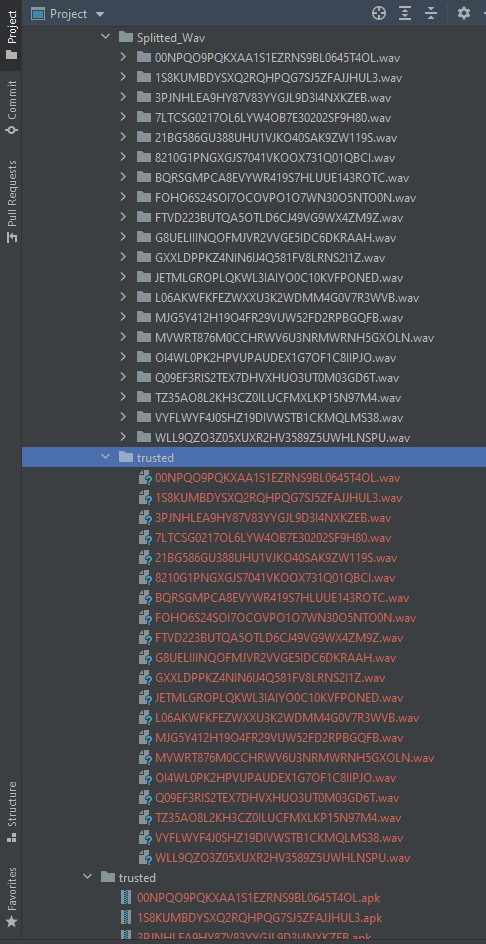
\includegraphics[width=0.9\linewidth, height= 6cm]{image/dirSplit.png} 
    \caption{cartelle create.csv}
    \label{fig:subim1}
    \end{subfigure}
    \begin{subfigure}{0.5\textwidth}
    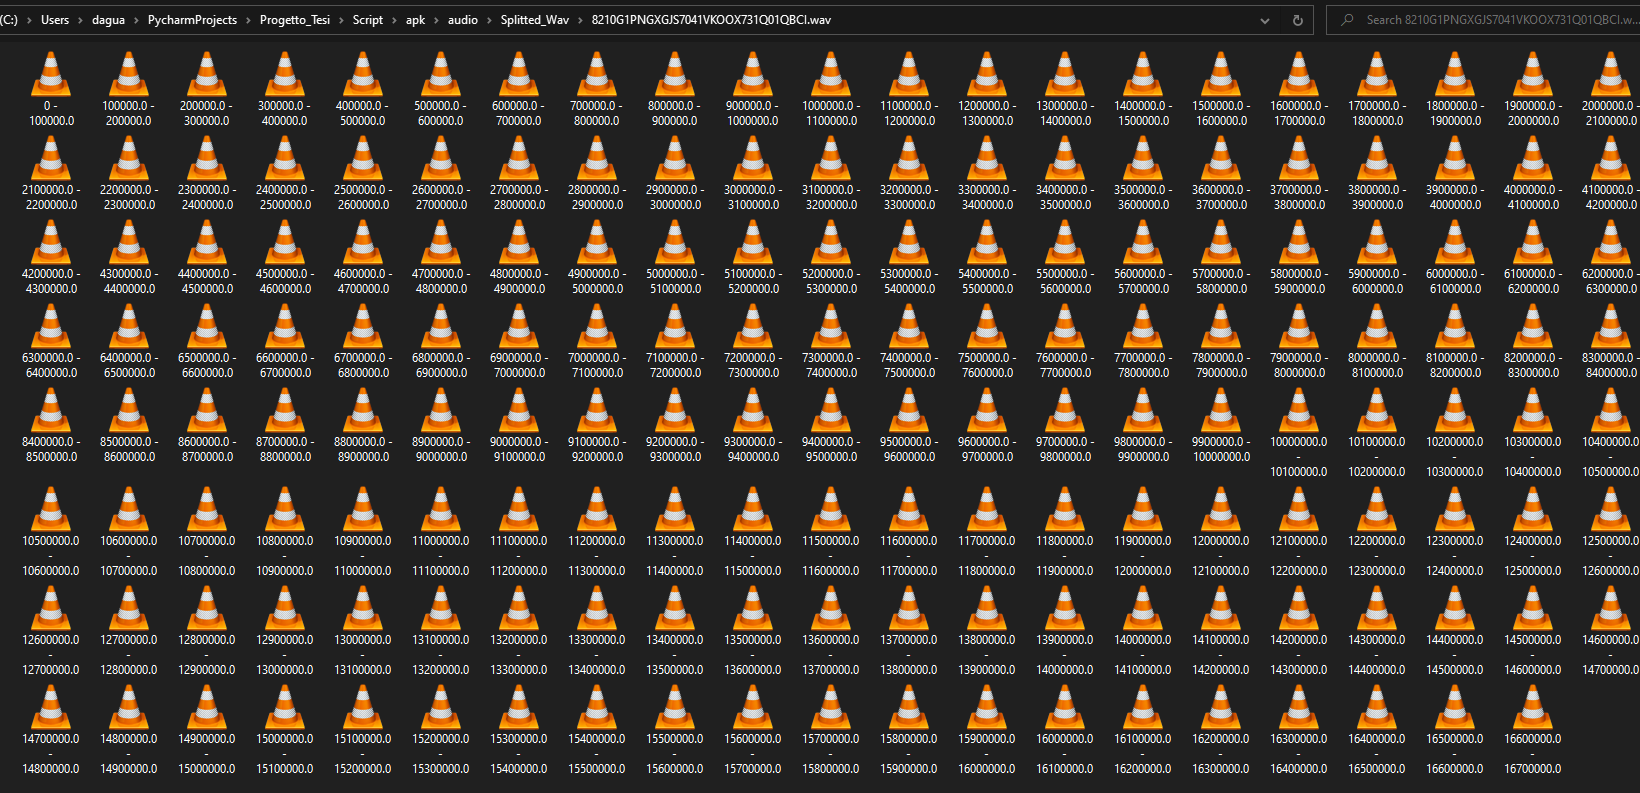
\includegraphics[width=0.9\linewidth, height= 3cm]{image/dirSplitted.png}
    \caption{wav creati }
    \label{fig:subim2}
    \end{subfigure}
    \caption{Subdirectory after scripts}
    \label{fig:image2}
    \end{figure}

\subsection{Library - wavSplitter.py}
    \begin{itemize}
        \item -   pip install pydub \url{https://github.com/jiaaro/pydub#installation}
        \item  
        \begin{enumerate}
            \item scaricare ffmpeg \url{https://www.gyan.dev/ffmpeg/builds/ffmpeg-release-full.7z}
            \item Estrarlo in una directory e aggiungere le path alle variabili di ambiente windows     \\\url{https://github.com/jiaaro/pydub/issues/348}
            \item pip install ffmpeg
        \end{enumerate}
    \end{itemize}

\section{Apk - Andorid App}
App tester sviluppate in API 29
L'apk va inserito in apk -> trusted
\\Il file APK non è altro che un archivio ZIP contenente tutto quello che serve alla nostra applicazione per funzionare
\begin{itemize}
    \item imamgini
    \item .xml
    \item META-INF contien il manifest con i permessi ed il certificato (firma)
    \item classes.dex
\end{itemize}

\section{Scripts - How Work}
\begin{enumerate}
   \item creare le cartelle nella cartella dove sono gli script 
    \begin{itemize}
        \item Script / apk / audio / trusted
        \\in questa cartella si andrà a generare il file .wav
        \item Script / apk / audio / malware
        \item Script / apk / malware 
        \item Script / apk / trusted 
        \\in questa cartella inseriamo l'applicazione \textbf{.apk}
    \end{itemize}
    \item eseguire lo script test.py
    \\genererà il file .wav 
    \item eseguire lo script progetto2.py
    \\genereraà il file .csv
    \begin{figure}[h]
    \begin{subfigure}{0.5\textwidth}
    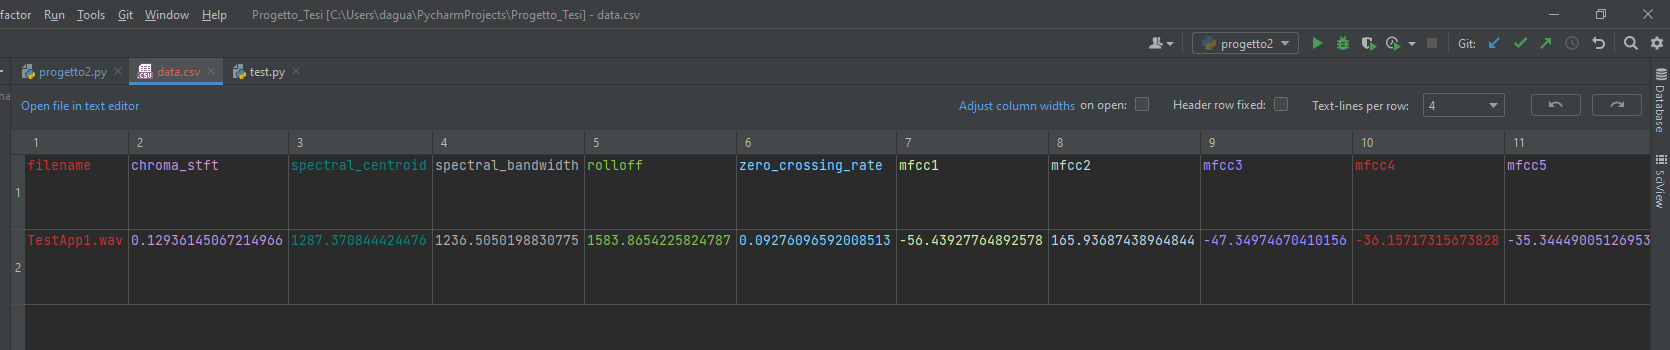
\includegraphics[width=0.9\linewidth, height=5cm]{image/Screenshot (34).png} 
    \caption{data.csv}
    \label{fig:subim1}
    \end{subfigure}
    \begin{subfigure}{0.5\textwidth}
    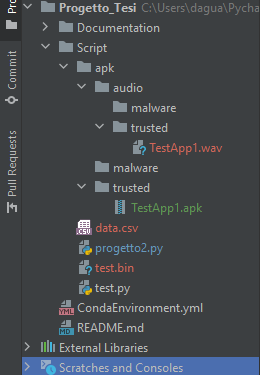
\includegraphics[width=0.9\linewidth, height=5cm]{image/Screenshot (33).png}
    \caption{wav generate}
    \label{fig:subim2}
    \end{subfigure}
    \caption{Subdirectory after scripts}
    \label{fig:image2}
    \end{figure}
\end{enumerate}


\end{document}
